% Slides for 2025-07-29
% To create a slide, use the following:
% \begin{frame}{TITLE}
%     BODY
% \end{frame}

% To create a slide with a bullet list, use the following:
% \begin{frame}{TITLE}
%     \begin{itemize}
%         \item ITEM 1
%         \item ITEM 2
%     \end{itemize}    
% \end{frame}

% To create a slide with numbered list, use the following:
% \begin{frame}{TITLE}
%     \begin{enumerate}
%         \item ITEM 1
%         \item ITEM 2
%     \end{enumerate}
% \end{frame}

% To create a slide with a graphic:
% 1. Add the graphic to this folder (named picture.png)
% 2. Use the following:
% \begin{frame}{TITLE}
%     \centering
%     \includegraphics[height=0.7\textheight,width=0.7\textwidth,keepaspectratio]{picture.png}
% \end{frame}

% To create a slide with two columns, use the following:
% \begin{frame}{TITLE}
%     \begin{columns}
%         \begin{column}{0.5\textwidth}
%             COLUMN 1 BODY
%         \end{column}
%         \begin{column}{0.5\textwidth}
%             COLUMN 2 BODY
%         \end{column}
%     \end{columns}
% \end{frame}

\begin{frame}{Hall Pass}
    \begin{enumerate}
        \item High-Level Recap
        \item HallPass A 
        \item HallPass B 
        \item HallPass C
        \item Next Steps
    \end{enumerate}
\end{frame}

\begin{frame}{High-Level Recap}
    \centering
    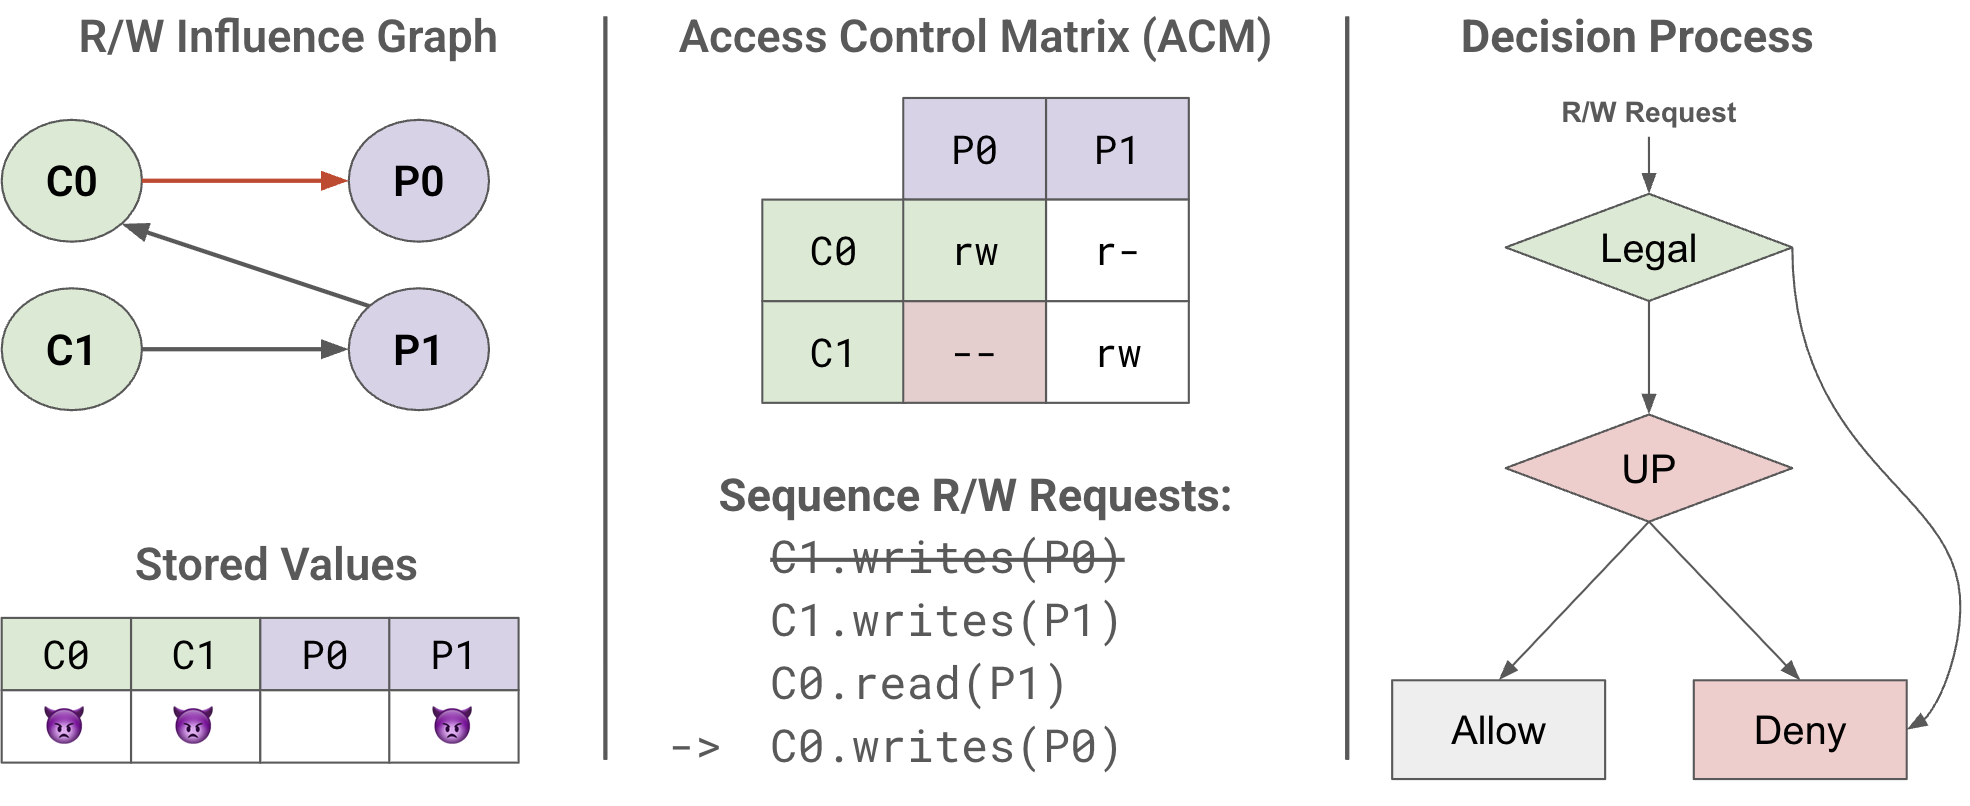
\includegraphics[height=0.95\textheight,width=0.95\textwidth,keepaspectratio]{images/hallpass_a.png}
\end{frame}

\begin{frame}{High-Level Recap}
    \centering
    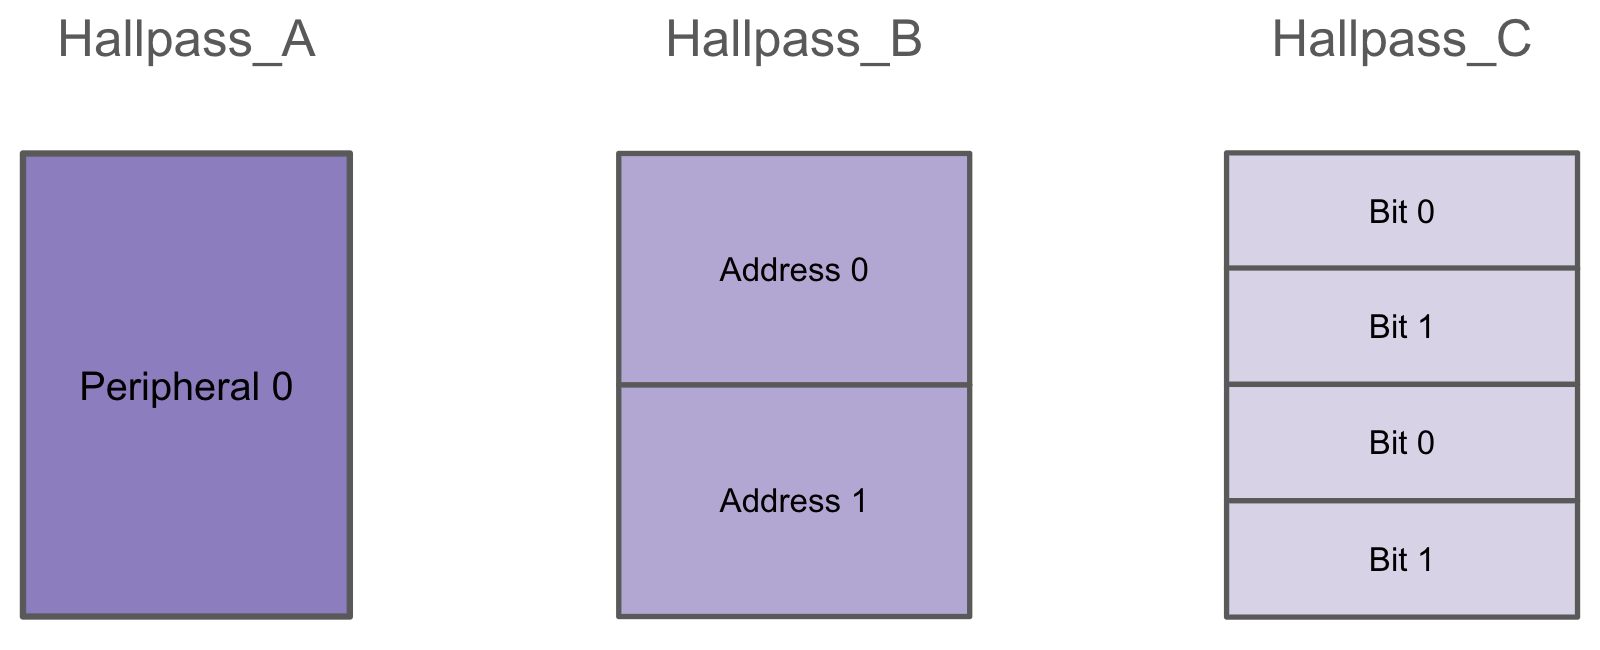
\includegraphics[height=0.95\textheight,width=0.95\textwidth,keepaspectratio]{images/intro.png}
\end{frame}

\begin{frame}{HallPass A}
    Highest level of performance \& lowest accuracy
    \begin{columns}
        \begin{column}{0.5\textwidth}
            \begin{itemize}
                \item Identifies unintended proxy at peripheral level
            \end{itemize}
            \centering
            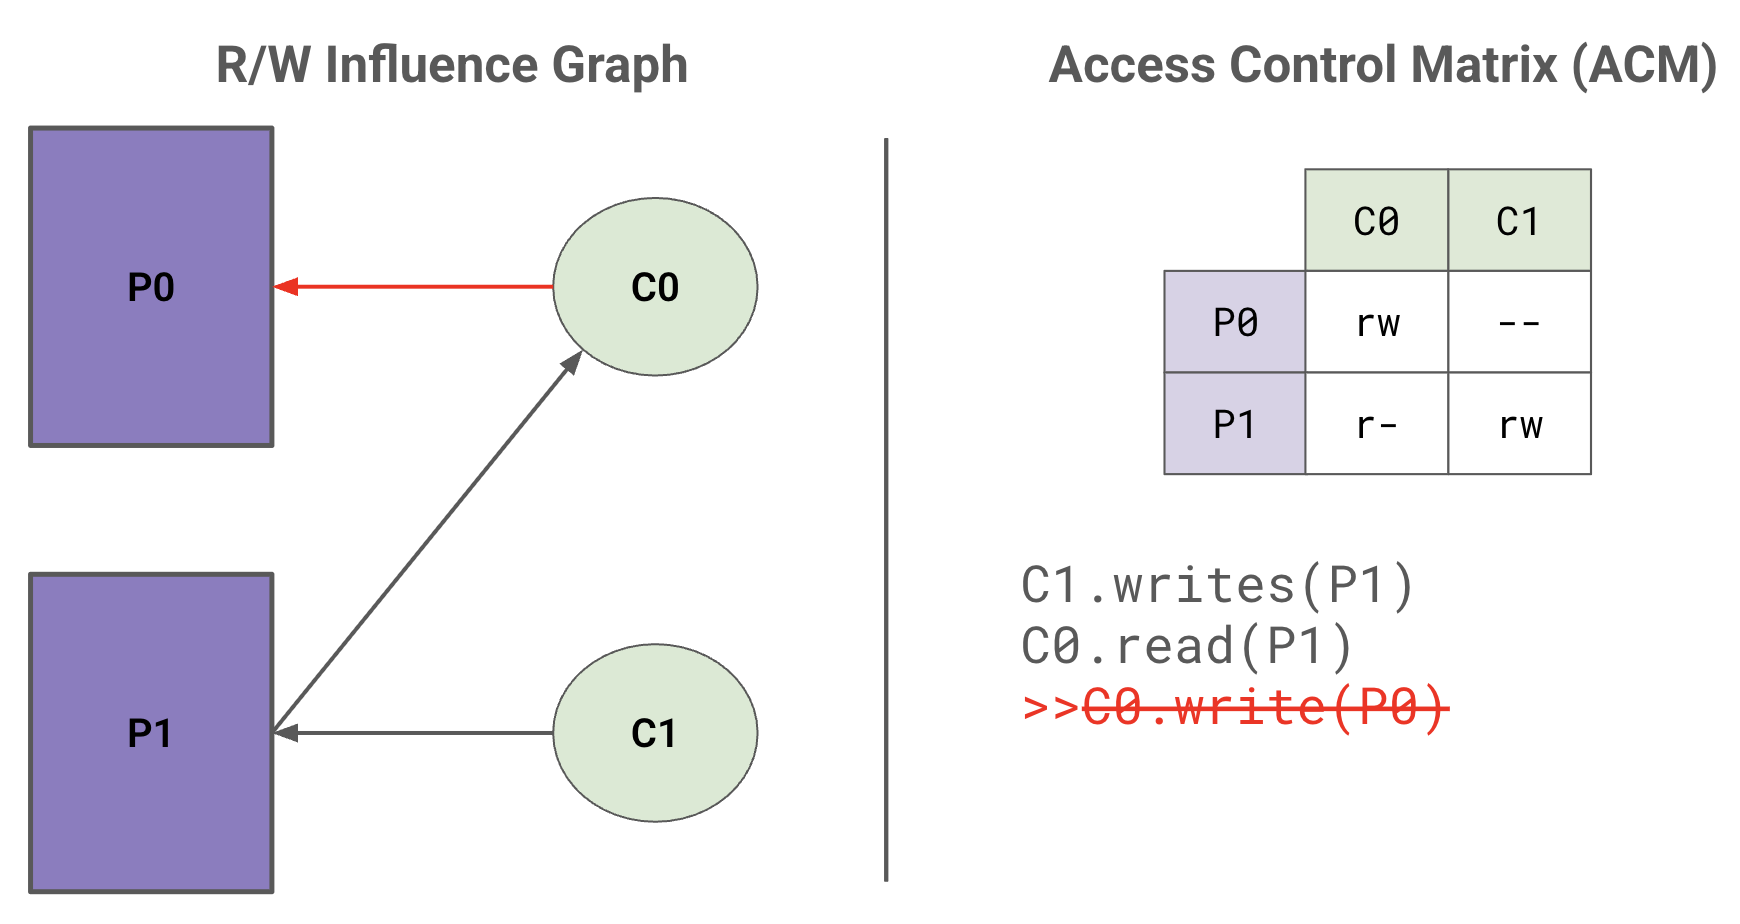
\includegraphics[height=0.7\textheight,width=0.7\textwidth,keepaspectratio]{images/hallpass_a_acm.png}
        \end{column}
    \end{columns}
\end{frame}

\begin{frame}{HallPass A}
    Highest level of performance \& lowest accuracy
    \begin{columns}
        \begin{column}{0.5\textwidth}
            \begin{itemize}
                \item Identifies unintended proxy at peripheral level
            \end{itemize}
            \centering
            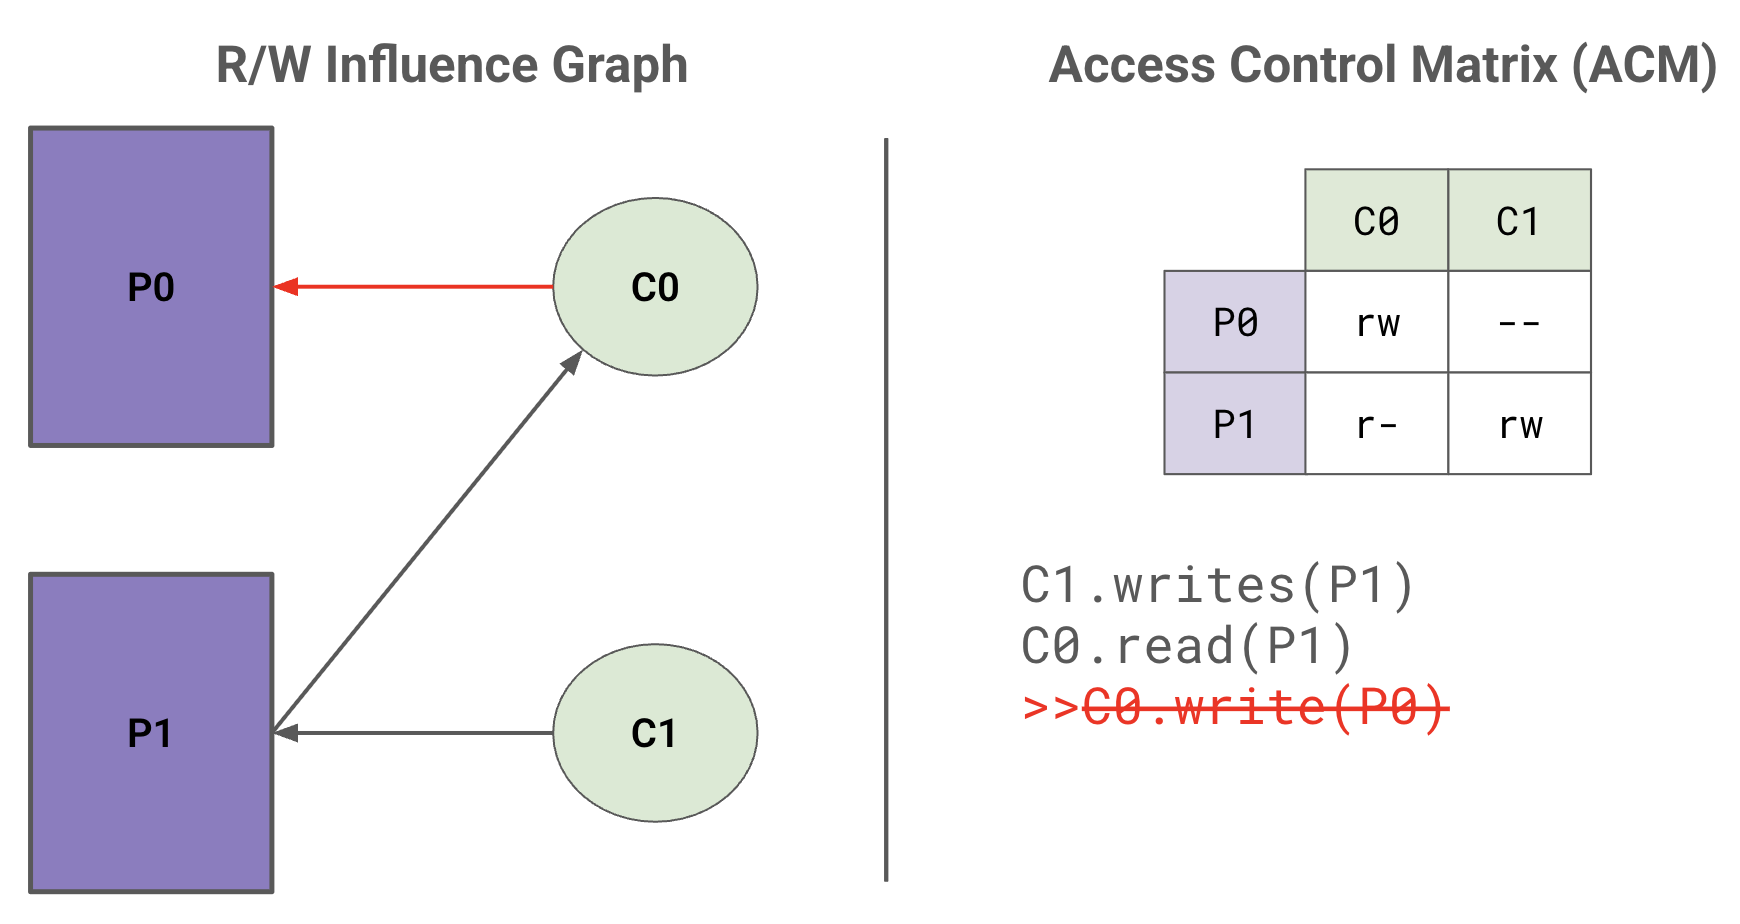
\includegraphics[height=0.95\textheight,width=0.95\textwidth,keepaspectratio]{images/hallpass_a_acm.png}
        \end{column}
       \begin{column}{0.5\textwidth}
            \begin{itemize}
                \item Optimises perfomance vs resource utilization
            \end{itemize}
            \centering
            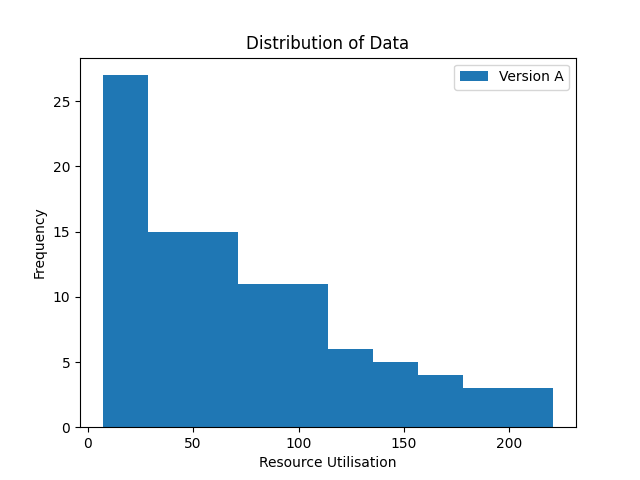
\includegraphics[height=0.5\textheight,width=0.5\textwidth,keepaspectratio]{images/hallpass_a_hist.png}
            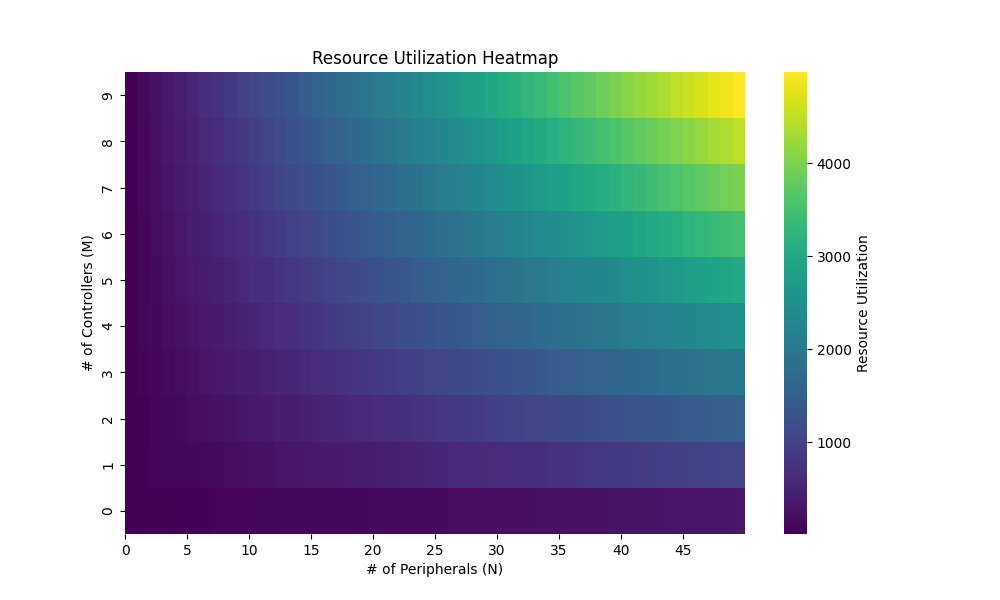
\includegraphics[height=0.5\textheight,width=0.5\textwidth,keepaspectratio]{images/hallpass_a_util.png}
       \end{column} 
    \end{columns}
\end{frame}

\begin{frame}{HallPass B}
    Moderate level of perfomance \& accuracy
            \begin{itemize}
                \item Identifies unintended proxy at address level
            \end{itemize}
            \centering
            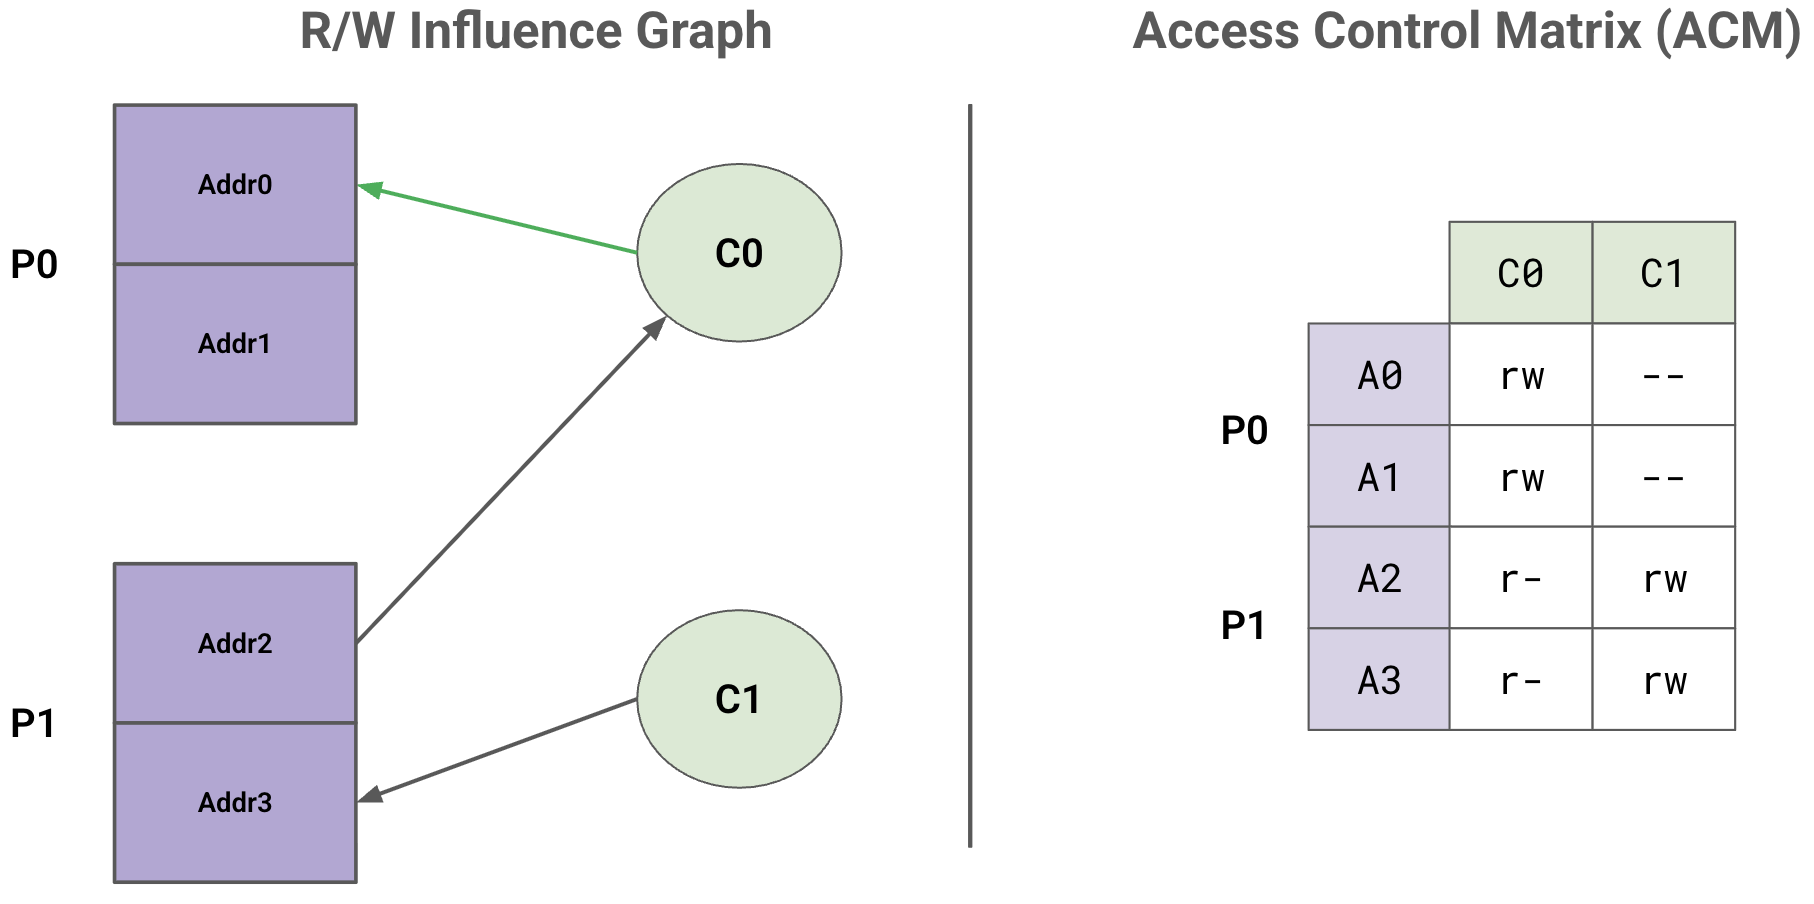
\includegraphics[height=0.85\textheight,width=0.85\textwidth,keepaspectratio]{images/halllpaass_b_slid1.png}
\end{frame}

\begin{frame}{HallPass B}
    Moderate level of perfomance \& accuracy
            \begin{itemize}
                \item Identifies unintended proxy at address level
            \end{itemize}
            \centering
            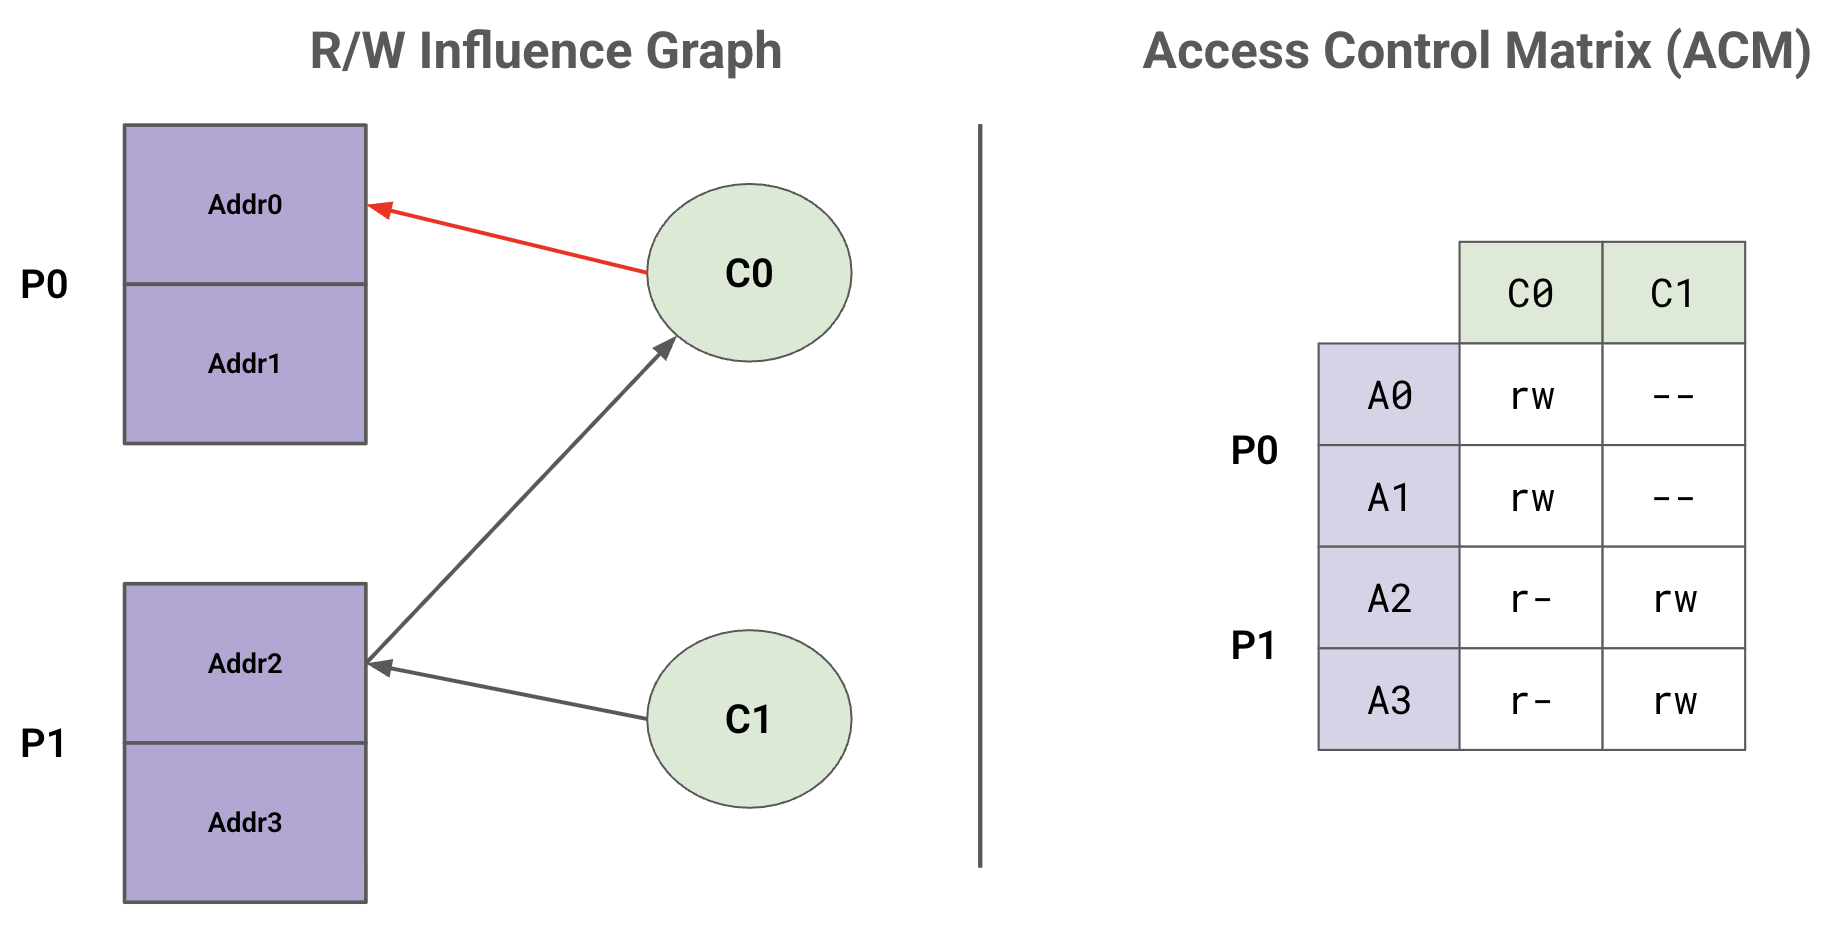
\includegraphics[height=0.85\textheight,width=0.85\textwidth,keepaspectratio]{images/hallpass_b_slid2.png}
\end{frame}

\begin{frame}{HallPass B}
    Moderate level of perfomance \& accuracy
    \begin{columns}
        \begin{column}{0.5\textwidth}
            \begin{itemize}
                \item More resource utilization than version A
            \end{itemize}
            \centering
            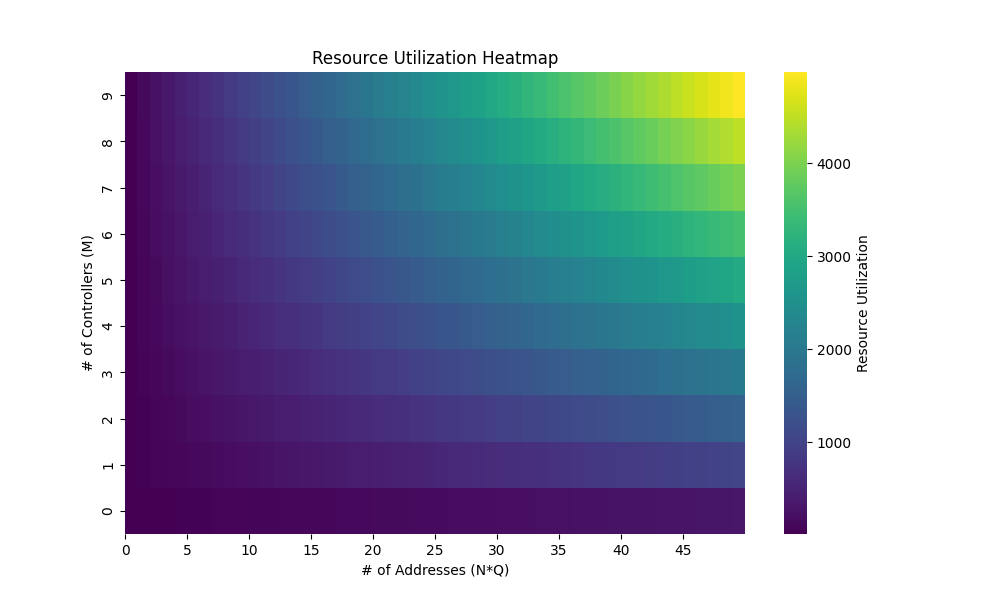
\includegraphics[height=0.85\textheight,width=0.85\textwidth,keepaspectratio]{images/hallpass_b_util.png}
        \end{column}
        \begin{column}{0.6\textwidth}
            \centering
            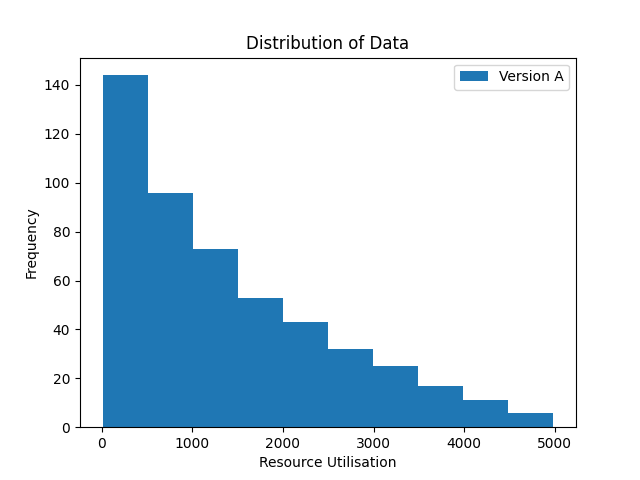
\includegraphics[height=0.85\textheight,width=0.85\textwidth,keepaspectratio]{images/hallpass_b_hist.png}
        \end{column}
    \end{columns}            
\end{frame}

\begin{frame}{HallPass C}
    Lowest level of perfomance \& highest accuracy
            \begin{itemize}
                \item Identifies unintended proxy at bit level
            \end{itemize}
            \centering
            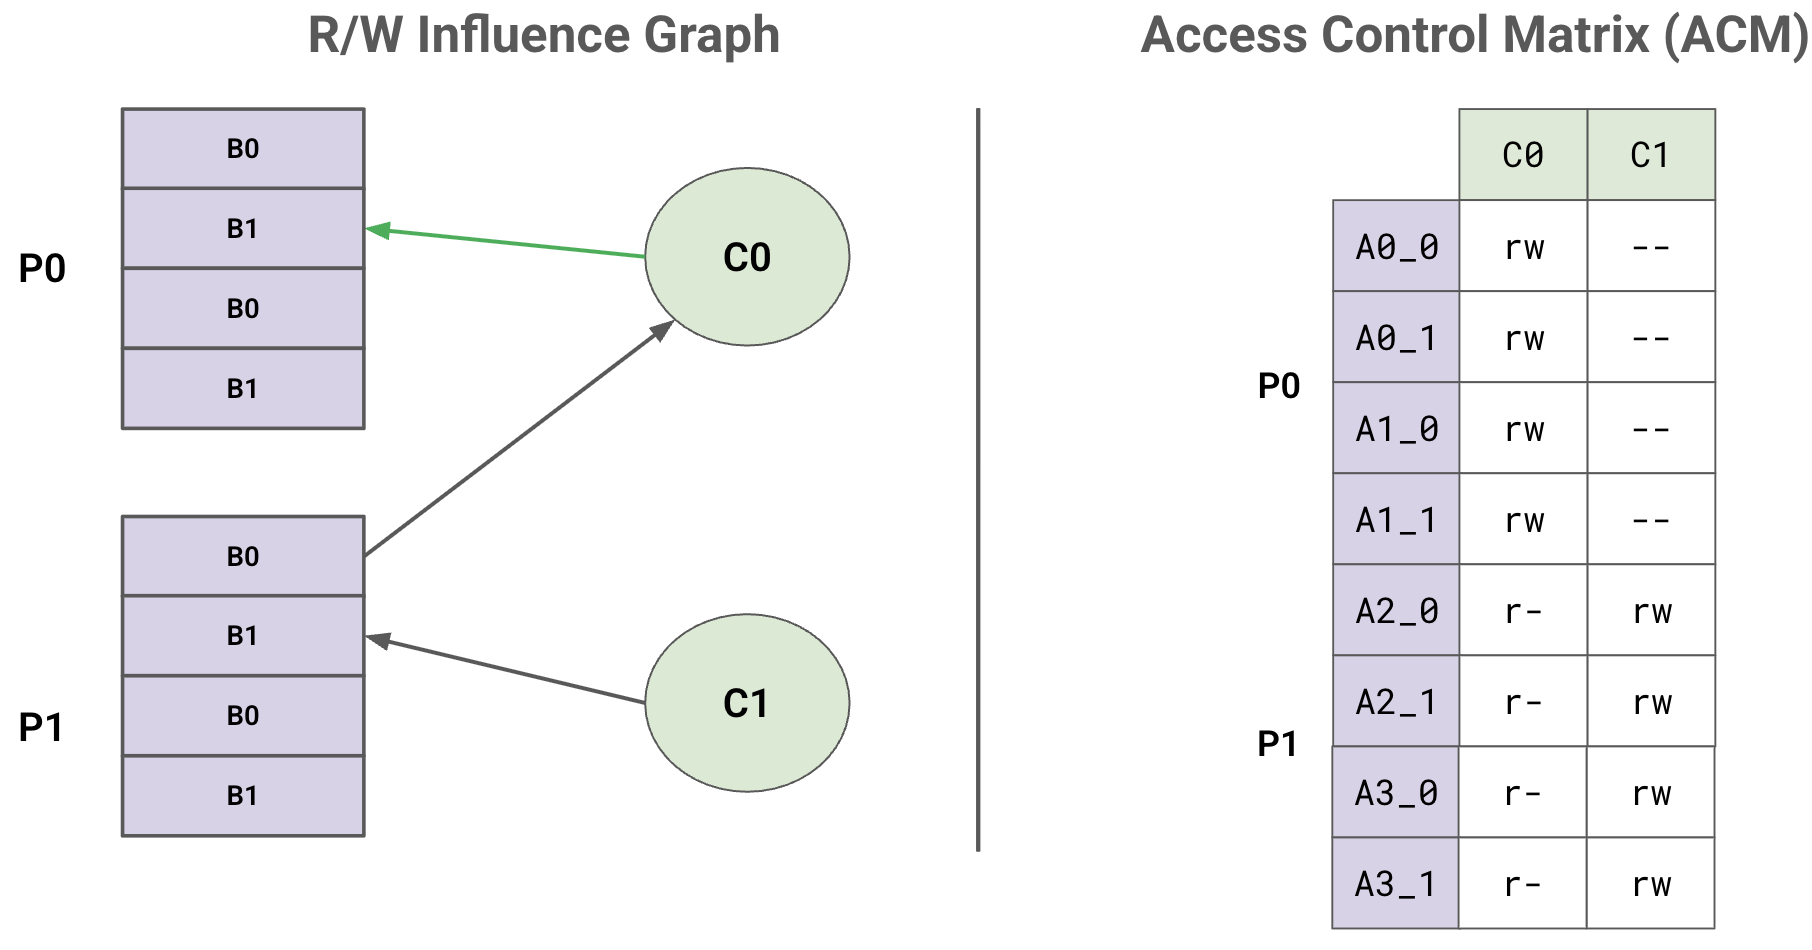
\includegraphics[height=0.85\textheight,width=0.85\textwidth,keepaspectratio]{images/hallpass_c_slid1.png}
\end{frame}

\begin{frame}{HallPass C}
    Lowest level of perfomance \& highest accuracy
            \begin{itemize}
                \item Identifies unintended proxy at bit level
            \end{itemize}
            \centering
            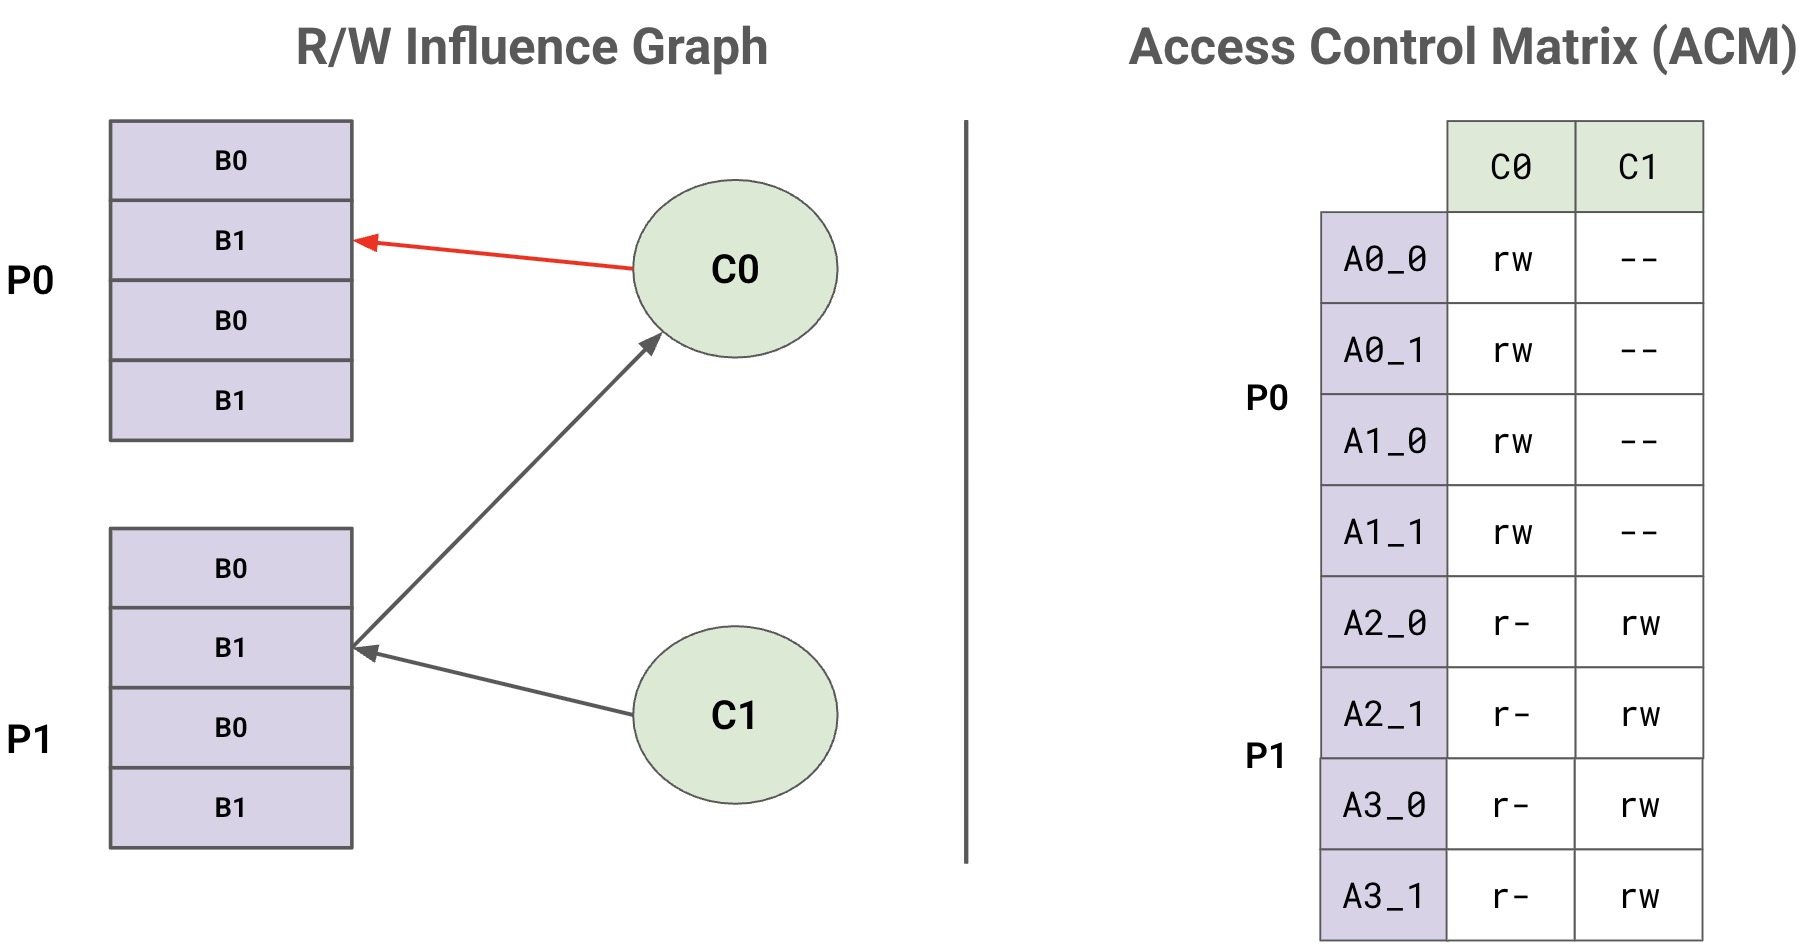
\includegraphics[height=0.85\textheight,width=0.85\textwidth,keepaspectratio]{images/hallpass_c_slid2.png}
\end{frame}

\begin{frame}{HallPass C}
    Lowest level of perfomance \& highest accuracy 
    \begin{columns}
        \begin{column}{0.5\textwidth}
            \begin{itemize}
                \item More resource utilization than version A and B
            \end{itemize}
            \centering
            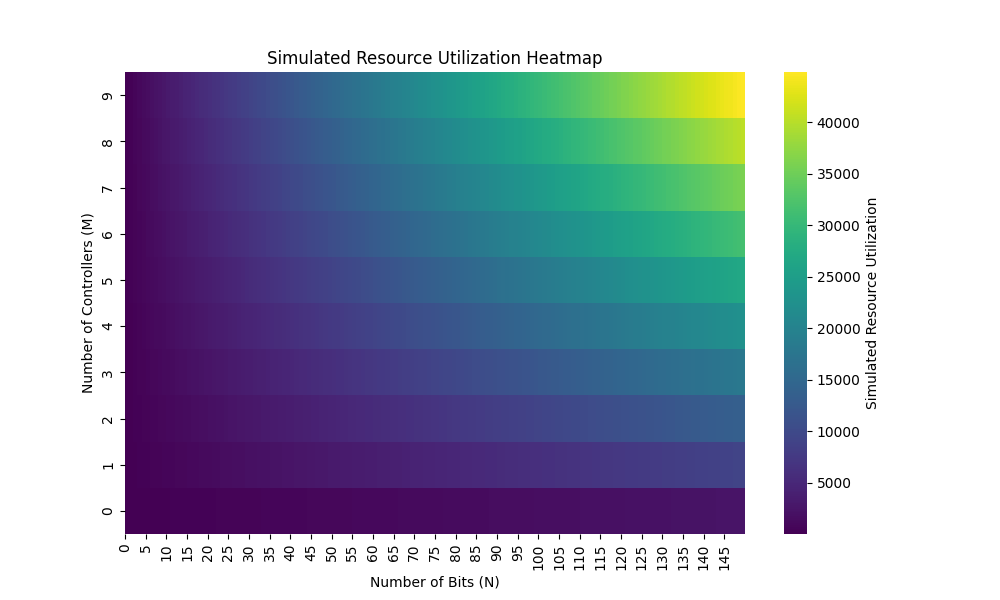
\includegraphics[height=0.85\textheight,width=0.85\textwidth,keepaspectratio]{images/10x10 heatmap HP_C.png}
        \end{column}
        \begin{column}{0.6\textwidth}
            \centering
            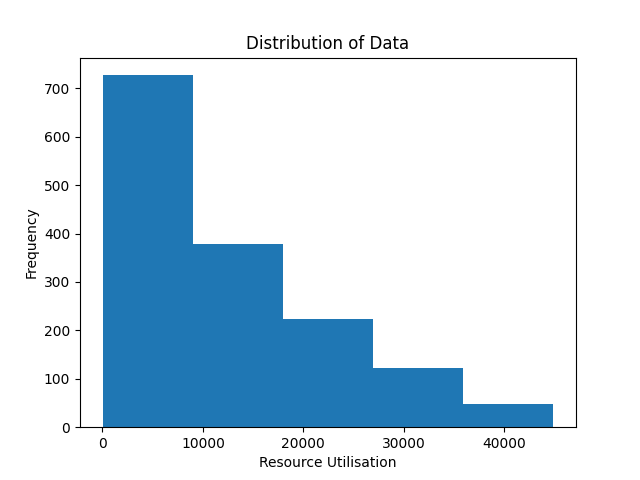
\includegraphics[height=0.85\textheight,width=0.85\textwidth,keepaspectratio]{images/10x10 histogram HP_C.png}
        \end{column}
    \end{columns}            
\end{frame}

\begin{frame}{Next Steps}
    \begin{enumerate}
        \item Code optimization and cleanup
        \item Calculate the rate of false positives in versions A and B
        \item Simulate the resource utilization in SystemVerilog with Vivado
    \end{enumerate}
\end{frame}